\uuid{6GaZ}
\exo7id{6954}
\auteur{ruette}
\organisation{exo7}
\datecreate{2013-01-24}
\isIndication{false}
\isCorrection{true}
\chapitre{Probabilité continue}
\sousChapitre{Autre}

\contenu{
\texte{
On considère un cercle. On choisit une corde au hasard et on cherche la
probabilité pour que cette corde passe à l'intérieur d'un triangle 
équilatéral inscrit dans le cercle dont un des sommets
est une des extrémités de la corde (voir la figure) ou, de façon équivalente,
pour que cette corde soit plus longue que le côté d'un triangle
équilatéral inscrit dans le cercle.

\bigskip
%\bigskip
\centerline{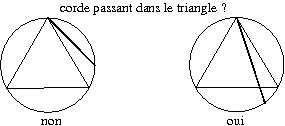
\includegraphics{../images/img006954-1}}


\bigskip
{\it Cet exercice est volontairement formulé de façon imprécise. Essayez
de trouver la solution de façon intuitive (pas de théorème à utiliser ici).
Il est fort probable que vous ne trouviez pas tous la même probabilité.
Historiquement, ce genre de paradoxe a motivé l'introduction d'une théorie
rigoureuse du hasard.
}
}
\reponse{
La corde $[AB]$ est déterminée par sa distance au centre $O$, qui
est $r=OM$, où $M$ est le milieu de $[AB]$,
et par l'angle $\theta$ entre l'horizontale et la droite $(OM)$
(voir la figure de gauche dans (1) ci-dessous). 
Le problème étant symétrique
par rotation, l'angle $\theta$ n'intervient pas. On est donc ramené à
choisir une distance $r$ au hasard dans $[0,R]$, où $R$ est le rayon du 
cercle. La corde est à l'extérieur si $r\geq r_0$ avec $r_0=\frac{1}{2}R$ 
(voir les figures (1) ci-dessous). Donc la probabilité cherchée est $1/2$
(on a pris la probabilité uniforme sur $[0,R]$).

\medskip
\centerline{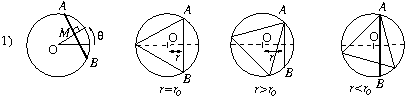
\includegraphics{../images/img006954-2}}
\medskip
La corde $[AB]$ est déterminée par son centre $M$ : il suffit de
tracer la perpendiculaire à $(OM)$ passant par $M$ (figure de gauche
ci-dessus, comme pour 1). On est donc ramené à choisir un point
$M$ au hasard dans le disque de rayon $R$.
La corde passe à l'intérieur du triangle
si $|OM|\leq \frac{1}{2}R$ (comme au 1), autrement
dit si le point $M$ se trouve dans le disque de rayon $R/2$, hachuré sur
la figure (2) ci-dessous.
L'aire du domaine est $\pi(R/2)^2$ et l'aire
totale est $\pi R^2$, donc la probabilité cherchée est $1/4$
(on a pris la probabilité uniforme sur le disque de rayon $R$).

\medskip
\centerline{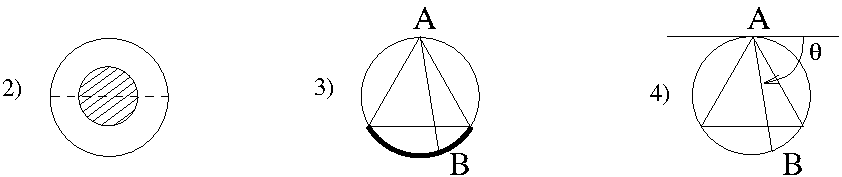
\includegraphics{../images/img006954-3}}
\bigskip
Une corde est déterminée par 2 points $A$ et $B$ 
sur le cercle (ses extrémités). Le problème étant symétrique par rotation,
on peut fixer le point $A$ et considérer la position du point $B$.
On est donc ramené à choisir un point $B$ au hasard sur le cercle.
La corde passe à l'intérieur du triangle pour $B$ appartenant à un arc
de cercle faisant 1/3 du cercle (voir la figure (3) ci-dessus).
Donc la probabilité cherchée est $1/3$
(on a pris la probabilité uniforme sur le cercle, c'est-à-dire la longueur
d'un arc divisé par la longueur du cercle entier).
On peut déterminer la corde par son extrémité $A$ et l'angle $\theta$ 
que fait la corde avec la tangente au cercle en $A$
(voir la figure (4) ci-dessus). On est donc ramené à choisir 
un angle $\theta$ au hasard dans $[0,\pi]$.
On voit que
la corde passe dans le triangle si $\pi/3\leq \theta\leq 2\pi/3$. Ce
qui donne une probabilité de $1/3$ (on a pris la probabilité
uniforme sur $[0,\pi]$).
}
}
